%\section {Définitions}

%
%  Robot
%

\begin{frame} {Robot}
  \centerline {
    \parbox{.66\linewidth} {
      Set of rigid bodies $\body_0,\cdots\body_m$, linked to one another by \textit{joints}.
      \vskip .5cm
      \centerline {
        \def\svgwidth {.5\linewidth}
        {\tiny
          \graphicspath{{./figures/}}
          \input {figures/kinematic-chain.pdf_tex}
        }
      }
      \vskip .5cm
      Joint~: parameterized rigid-body transformation between two frames (in SE(3)).
    }
    \parbox {.33\linewidth} {
      \centerline {
        \includegraphics[width=\linewidth]{figures/hrp2.jpg}
      }
    }
  }
\end{frame}

%
%  Déplacement rigide
%

\begin {frame} {Rigid body transformation}
  Definitions
  \begin {itemize}
  \item SO(3)~: group of 3 by 3 rotation matrices.
   $$R\in SO(3) \Leftrightarrow R^TR = I_3\ \mbox{and}\ \det(R)=1$$
  \item SE(3)~: group of rigid body tranformations
    \begin{eqnarray*}
      T\in SE(3) \Leftrightarrow && \exists t\in\real^3, \exists R\in SO(3)\\
      && \forall x\in\real^3\ T(x) = Rx + t
    \end{eqnarray*}
    We denote $T = T_{(R,t)}$.
  \end{itemize}
\end{frame}

%
%  Articulation
%
\begin {frame} {Joint}
  A joint is represented by a mapping from a sub-manifold of $\real^p$ in SE(3),
  where $p\geq 1$ is an integer.\\
  Examples~:\\
  \centerline {
    \parbox {.5\linewidth} {
      \begin {itemize}
      \item Translation T1~:
        \begin{eqnarray*}
          \real & \rightarrow & SE(3) \\
          t & \rightarrow & T_{(I_3, (t\ 0\ 0))}
        \end{eqnarray*}
      \end {itemize}
      \vskip .5cm
    }
    \parbox {.49\linewidth} {translation along x}
  }
\end {frame}

%
%  Articulation
%
\begin {frame} {Joint}
  A joint is represented by a mapping from a sub-manifold of $\real^p$ in SE(3),
  where $p\geq 1$ is an integer.\\
  Examples~:\\
  \centerline {
    \parbox {.5\linewidth} {
      \begin {itemize}
      \item Translation T3~:
        \begin{eqnarray*}
          \real^3 & \rightarrow & SE(3) \\
          t & \rightarrow & T_{(I_3, t)}
        \end{eqnarray*}
      \end {itemize}
      \vskip .5cm
    }
    \parbox {.49\linewidth} {translation}
  }
\end {frame}

%
%  Articulation
%
\begin {frame} {Joint}
  A joint is represented by a mapping from a sub-manifold of $\real^p$ in SE(3),
  where $p\geq 1$ is an integer.\\
  Examples~:\\
  \centerline {
    \parbox {.5\linewidth} {
      \begin {itemize}
      \item Rotation R1~:
        \begin{eqnarray*}
          \real & \rightarrow & SE(3) \\
          t & \rightarrow & T_{(R, 0)}
        \end{eqnarray*}
      \end {itemize}
      \vskip .5cm
    }
    \parbox {.49\linewidth} {
      $$ R=\left(\begin{array}{ccc}\cos t & -\sin t & 0 \\ \sin t & \cos t & 0 \\ 0&0&1\end{array}\right)$$
    }
  }
\end {frame}

%
%  Articulation
%
\begin {frame} {Joint}
  A joint is represented by a mapping from a sub-manifold of $\real^p$ in SE(3),
  where $p\geq 1$ is an integer.\\
  Examples~:\\
  \centerline {
    \parbox {.5\linewidth} {
      \begin {itemize}
      \item Rotation R3~:
        \begin{eqnarray*}
          \real^4 & \rightarrow & SE(3) \\
          t & \rightarrow & T_{(R, 0)}
        \end{eqnarray*}
      \end {itemize}
      \vskip .5cm
    }
    \parbox {.49\linewidth} {
      {\tiny
        $$
          \|t\| = 1
          $$
          $$\begin{array}{c}R=\\
          \left(\begin{array}{ccc}1 - 2(t_2^2 + t_3^2) & 2t_2t_1 - 2t_3t_0 & 2t_3t_1 + 2t_2t_0\\ 2t_2t_1 + 2t_3t_0 & 1 - 2(t_1^2 + t_3^2) & 2t_3t_2 - 2t_1t_0\\ 2t_3t_1 - 2t_2t_0 & 2t_3t_2 + 2t_1t_0 & 1 - 2(t_1^2 + t_2^2)\end{array}\right)\end{array}$$
          $$t_0 + t_1 i + t_2 j + t_3 k\ \mbox{is a quaternion.}$$
      }
    }
  }
\end {frame}

%
%  Quaternion
%
\begin {frame} {Quaternions}
  \centerline {
    \parbox {.75\linewidth} {
      Non-commutative field isomorphic to $\real^4$, spanned by three elements
      $i, j, k$ that satisfy the following relations~:
      $$i^2 = j^2 = k^2 = ijk = -1$$
      \pause
      from which we immediately deduce
      $$ ij=k,\ jk=i,\ ki=j$$
    }
    \parbox {.24\linewidth} {
      \includegraphics [width=\linewidth] {pictures/William_Rowan_Hamilton_painting.jpg}\\
      \centerline {Hamilton (1843)}
    }
  }
\end {frame}

%
%  Quaternions unitaires et rotations
%
\begin {frame} {Unit Quaternions and rotations}
  Let $q=q_0 + q_1 i + q_2 j + q_3 k$ be a unit quaternion:
  $$q_0^2 + q_3^2 + q_2^2 + q_3^2 = 1$$
  \pause
  $\forall x = (x_0, x_1, x_2)\in\real^3$, let $u=x_0i + x_1 j + x_2 k$
  $$
  q\,.\,u\,.\,q^* = y_0 i + y_1 j + y_2 k
  $$
  where $q^*=q_0 - q_1 i - q_2 j - q_3 k$ is the conjugate of $q$.\\
  \pause
  $y = (y_0, y_1, y_2)$ is the image of $x$ by the rotation of matrix
  $$
  \left(\begin{array}{ccc}1 - 2(q_2^2 + q_3^2) & 2q_2q_1 - 2q_3q_0 & 2q_3q_1 + 2q_2q_0\\ 2q_2q_1 + 2q_3q_0 & 1 - 2(q_1^2 + q_3^2) & 2q_3q_2 - 2q_1q_0\\ 2q_3q_1 - 2q_2q_0 & 2q_3q_2 + 2q_1q_0 & 1 - 2(q_1^2 + q_2^2)\end{array}\right)
  $$
\end{frame}

%
%  Quaternions unitaires et rotations
%
\begin {frame} {Unit Quaternions and rotations}
  \begin{itemize}
    \item Notice that $q$ and $-q$ represent the same rotation
    \item $SO(3)$ is isomorphic to $Sp(1)/\{\pm 1\}$, the half-sphere of
      $\real^4$.
  \end{itemize}
\end{frame}

%
%  Configuration d'un robot
%
\begin {frame} {Configuration of a robot}
  \centerline {
    \parbox{.66\linewidth} {
      The configuration $\conf$ of a robot is represented by the concatenation
      of the parameters of each joint.
      \vskip .5cm
      \centerline {
        \def\svgwidth {.5\linewidth}
        {\tiny
        \graphicspath{{./figures/}}
        \input {figures/kinematic-chain.pdf_tex}
        }
      }
    }
    \parbox {.33\linewidth} {
      \centerline {
        \includegraphics[width=\linewidth]{figures/hrp2.jpg}
      }
    }
  }
\end {frame}

%
%  Cinématique directe
%
\begin {frame} {Forward kinematics}
  \centerline {
    \parbox{.66\linewidth} {
      Computation of the position of each joint in the global frame
      $$
      M_i (\conf) = M_{parent (i)} (\conf)\ M_{i/parent}\ T_i (\conf)
      $$
      \centerline {
        \def\svgwidth {\linewidth}
        {\tiny
        \graphicspath{{./figures/}}
        \input {figures/forward-kinematics.pdf_tex}
        }
      }
    }
    \parbox {.33\linewidth} {
      \centerline {
        \includegraphics[width=\linewidth]{figures/hrp2.jpg}
      }
    }
  }
\end{frame}

%
%  Obstacle
%

\begin{frame} {Definitions}

\begin{itemize}
\item Workspace: $\WS=\real^2$ or $\real^3$: space in which the robot evolves
\pause
\item Obstacle in workspace: compact subset of $\WS$, denoted by $\obst$.
\pause
\item Configuration space: $\CS$.
\pause
\item Position in configuration $\conf$ of a point $M\in\body_i$:
  $\x_i(M,\conf)$.
\pause
\item Obstacle in the configuration space:
\begin{eqnarray*}
\CSobst&=\{\conf\in\CS,&\exists i\in\{1,\cdots,m\},\ \exists M\in\body_i,\ \x_i(M,\conf)\in\obst\ \mbox{or}\\
&&\exists i,j\in\{1,\cdots,m\},\ \exists M_i\in\body_i,\ \exists M_j\in\body_j,\\
&&\x_i(M_i,\conf)=x_j(M_j,\conf)\}
\end{eqnarray*}
\pause
\item Free configuration space: $\CSfree = \CS\setminus\CSobst$.
\end{itemize}
\end{frame}

%
%  Motion
%

\begin{frame} {Motion}

\begin{itemize}
\item Configuration space:
  \begin{itemize}
  \item differential manifold
  \end{itemize}
  \pause
\item Motion:
  \begin{itemize}
  \item continuous function from $[0,1]$ to $\CS$.
  \end{itemize}
  \pause
\item Collision-free motion:
  \begin{itemize}
  \item continuous function from $[0,1]$ to $\CSfree$.
  \end{itemize}
\end{itemize}
\end{frame}

%
%  Motion planning
%

\begin{frame} {Motion planning problem}
  \parbox{.49\linewidth}{
    \centerline{
      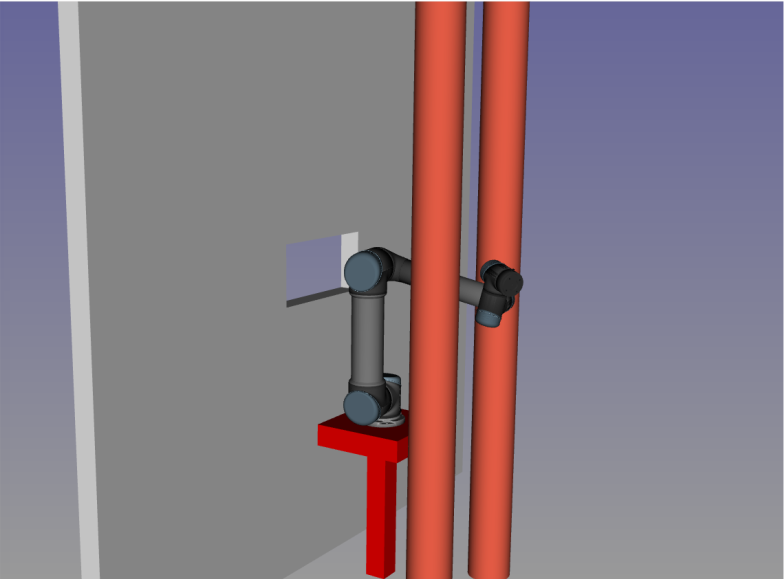
\includegraphics[width=\linewidth]{figures/motion-planning-init.png}
    }
    \centerline{initial configuration}
  }
  \parbox{.49\linewidth}{
    \centerline{
      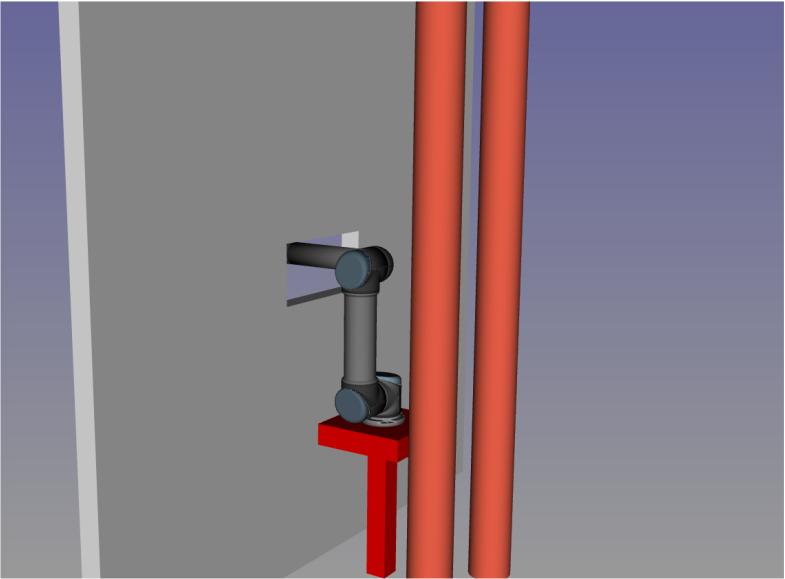
\includegraphics[width=\linewidth]{figures/motion-planning-goal.png}
    }
    \centerline{goal configuration}
  }
  \vskip .5cm
  \centerline{$\CS=\real^6$}
\end{frame}
